\documentclass[a4paper, 11pt]{article}

\usepackage{amsmath, amssymb, amstext, amsfonts, mathrsfs}	% Mathe
\usepackage{hyperref}		%Anklicken von Links
\usepackage[normalem]{ulem}	%weitere Formatierung von Schriften
\usepackage{fancyhdr}		%sch\"one Kopf- und Fußzeilen
\usepackage{verbatim}
\usepackage{graphicx}
\usepackage[]{algorithm2e}

\pagestyle{fancy}
\lhead{Data-driven intelegent systems\\}
\chead{\ \\Florian Vahl}
\rhead{\today\\}

\parindent0pt

\begin{document}
\section{Task}

\subsection{Manual tree generation}

First we calculate the Entropy over all labels
\begin{equation}
    Info(D) = I(5,3) = -\frac{5}{8}\log_2(\frac{5}{8}) - \frac{3}{8}\log_2(\frac{3}{8}) = 0.954
\end{equation}

Than we calculate the Entropy and the Information Gain for the class weather
\begin{equation}
    Info_{weather}(D) = \frac{4}{8}I(4,0) + \frac{4}{8}I(1,3) = \frac{4}{8}*0 + \frac{4}{8} * 0.811 = 0.4
\end{equation}

\begin{equation}
    Gain_{weather}(D) = Info(D) - Info_{weather}(D) = 0.954 - 0.4 = 0.554
\end{equation}

And for the class hungry
\begin{equation}
    Info_{hungry}(D) = \frac{4}{8}I(3,1) + \frac{4}{8}I(2,2) =  \frac{4}{8}*0.811 + \frac{4}{8} * 1 = 0.905
\end{equation}

\begin{equation}
    Gain_{hungry}(D) = Info(D) - Info_{hungry}(D) = 0.954 - 0.905 = 0.0485
\end{equation}

A split along the 'weather' results in the highest information gain. Therefore the first decision checks wether it is sunny or rainy.

Do we need further checks/nodes if it is sunny?

\begin{equation}
    Info(D) = I(4,0) = 0
\end{equation}

Because the entropy is zero in the training data set after the weather split on the sunny side of the tree nothing can be gained.
\\
For the rainy side

\begin{equation}
    Info(D) = I(1,3) = -\frac{1}{4}\log_2(\frac{1}{4}) - \frac{3}{4}\log_2(\frac{3}{4}) = 0.811
\end{equation}
\begin{equation}
    Info_{hungry}(D) = \frac{1}{2}I(1,1) + \frac{1}{2}I(0,2) =  \frac{1}{2}*1 + \frac{1}{2} * 0 = 0.5
\end{equation}
\begin{equation}
    Gain_{hungry}(D) = Info(D) - Info_{hungry}(D) = 0.811 - 0.5 = 0.311
\end{equation}

This results in another split by the hungry parameter after the rainy decision.

\begin{figure}[h!]
    \centering
    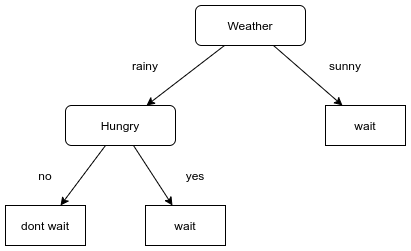
\includegraphics[width=\linewidth]{fig/ID3Tree.png}
    \caption{The generated ID3 Tree.}
    \label{fig:tree}
\end{figure}

\subsection{Questions}

\begin{itemize}
    \item For which kind of data you can use a decision tree?

    The data should have predefined discrete classes. It should also be labeled.
    The data type itself depends on the used tree, but most ones process discrete or continuos data.

    \item What is the learning strategy in a decision tree?

    The tree uses a greedy supervised learning algorithm.

    \item What is \textit{entropy} in this context and why is it necessary to compute?

    Measure of uncertainty associated with an in this case discrete random variable.
    In this case the entropy is used to describe the information that is associated with an parameter label combination.
\end{itemize}

\section{Task}

I ran the decision tree code, had a look at every step and played a bit with it.
\\
In this context Gini index referrers to the Gini Impurity describing the label distribution in a set.
It is larger if the labels more distributed.
Therefore good splits result lower a Gini index and more consistent classification after the split.

\section{Task}

The intended perceptron should divide the input space as shown in figure~\ref{fig:perceptron_space}

\begin{figure}[h!]
    \centering
    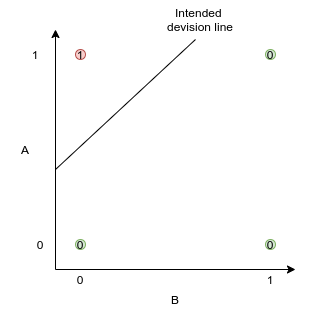
\includegraphics[width=0.5\linewidth]{fig/Perecpt_graph.png}
    \caption{Input space with annotations and the intended division by the perceptron.}
    \label{fig:perceptron_space}
\end{figure}

Our perceptron is designed with the following points in mind.
A strong negative weight of the B input results in an inhibitory behavior.
Meaning, that if B is activated the perceptrons output pulled down to negative values, resulting in an output of zero as intended.
The given formula outputs true iff B is false and A true.
If both inputs are zero the output needs to be negative, so a negative bias of -0.1 is applied.
The weight of A is intentionally lower than the weight of B, so if both are activated B wins and the output is zero.
A output is therefore only positive if A is positive (it contributes a positive value after multiplication with the weight), B is zero (the weight can be ignored in this case) and the contribution of A is larger than the bias.
This results in the possible values shown in figure~\ref{fig:perceptron}.

\begin{figure}[h!]
    \centering
    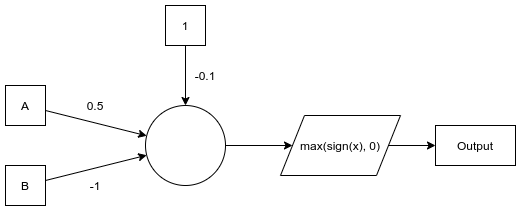
\includegraphics[width=0.9\linewidth]{fig/Perecpt.png}
    \caption{The developed perceptron.}
    \label{fig:perceptron}
\end{figure}

\newpage

\section{Task}

\begin{algorithm}[H]
 \KwData{\\
     $e^{(train)} = 1$\;
     $epoch = 0$\;
     $v_{ij} = rand(0,1)$\;
     $w_{jk} = rand(0,1)$\;
     $learning\_rate$ This value is set by the user\;
     $loss\_goal$ This value is set by the user\;
     $max\_epoch$ This value is set by the user\;
 }
 \While{$e^{(train)} > loss\_goal \indent \lor \indent epoch < max\_epoch$}{
  all temporary weight-updates $\Delta v_{ij} = \Delta w_{jk} = 0$\;
  overall sum-of-squares training error: $e^{(train)} = 0$\;
  \For{each data point $d$}{
    activations of input neurons $i$: $x_i = x_i^{(d)}$\;
    activations of hidden neurons $j$: $a_j = \frac{1}{1 + exp(-(-1 + \sum_i v_{ij}x_i))}$\;
    activations of output neurons $k$: $y_k =\frac{1}{1 + exp(-(-1 + \sum_j w_{jk}a_j))}$\;
    error for output neurons $k$: $\delta_k = y_k*(1-y_k)*(y_k^{(d)} - y_k)$\;
    error for hidden neurons $j$: $\delta_j = a_j*(1-a_j)*\sum_k \delta_k w_{jk}$\;
    cumulative updates for output neuron weights: $\Delta w_{jk} += \delta_k * a_j$\;
    cumulative updates for hidden neuron weights: $\Delta v_{ij} += \delta_j*x_i$\;
    sum overall error: $e^{(train)} += (y_k^{(d)} - y_k)^2$\;
  }
  adapt weights: \\
  $v_{ij} += learning\_rate * \Delta v_{ij},$\\ $w_{jk} += learning\_rate * \Delta w_{jk}$\;
  increase epoch count: $epoch++$\;
 }
 \caption{Simple MLP training with backpropagation.}
 \label{alg:mpl}
\end{algorithm}

The learning rate and the bias where missing in the original pseudocode.
The corrected code~\ref{alg:mpl} includes both of them.
Additionally the sum error is now squared and and the termination criteria is now more realistic, because an error of 0 is not expectable in noisy data.
Such a low training error could also easily be overfitted. Therefore two parameters (max epoch and max error) had been introduced.


\end{document}



















